%!TEX root = ../Bachelorarbeit.tex
\chapter{Architektur des Backends}

In diesem Kapitel wird das Backend-Konzept von Project-Zoom betrachtet. Begonnen wird mit einem Überblick über den Anwendungsaufbau. Anschließend wird ein konkretes Datenmodell entworfen, um daraufhin mit dem data-centric Design ein Konzept zur Umsetzung dieses Modells zu verdeutlichen.  Den Abschluss bildet ein weiterer Teil der Architektur, das Eventsystem.
%--------------------------------------------------------------------------------------------------------------------------------------------

\section{Anwendungsart}
\subsection{Webanwendung vs. native Applikation}
Eine grundlegende Entscheidung im Entwurf betrifft die Art der Anwendung. Für dieses Projekt kommen eine Webanwendung oder eine native Anwendung in Frage. 

Auf Grund der Anforderung der D-School, dass die Anwendung auch außerhalb der Räumlichkeiten der D-School verfügbar sein muss (vgl. Anforderung \ref{itm:f6}), liegt eine Webanwendung nahe. Hinzu kommt, dass die Projektmitglieder bereits mit dem Umgang von Webseiten und deren Navigation vertraut sind. Für die Erweiterbarkeit stellt dies ebenfalls einen enormen Vorteil dar, da ein zentrales System gewartet werden kann und neue Funktionen einfach eingespielt werden können. Zudem dreht sich das Projekt um das Thema Dokumentation, bei welchem oft dazu geneigt wird, es aufzuschieben. Eine Webseite senkt hier die Hemmschwelle und umgeht die Notwendigkeit einer Verteilung und Installation eines Programms.

Eine Trennung der Applikation in Frontend und Backend erlaubt eine klare Funktionstrennung. Für Webapplikationen befindet sich das Backend auf Serverseite und das Frontend im Browser auf Clientseite. Die klassischen Aufgaben der beiden Teile sind:  
\setstretch{1.2} %FIX
\paragraph{Backend-Aufgaben}
\begin{itemize}
  \item Sammeln und zur Verfügung stellen von Daten
  \item Kommunikation mit anderen Servern
  \item Validierung eingehender Daten vom Client
  \item Speicherung von Daten
  \item Business-Logik
\end{itemize}

\paragraph{Frontend-Aufgaben}
\begin{itemize}
  \item Kommunikation mit dem Backend zur Daten-Synchronisation 
  \item Visualisierung der Daten
  \item Interaktion mit dem Nutzer
  \item Feedback an den Nutzer
\end{itemize}
\setstretch{1.3} %FIX
\subsection{Generelle Architektur von Webapplikation-Backends}

Die grundlegende Architektur beim Bau einer Webanwendung hängt bei der Wahl eines Webframeworks vom Stil dieses Frameworks ab. Die Verwendung eines Webframeworks erlaubt die Konzentration auf die Umsetzung der Webschnittstelle und beschleunigt die Programmierung von Webanwendungen durch das Forcieren von Prinzipien wie "Don't repeat yourself" (vgl. \cite[p.~23]{pragmatic-programmer}) oder "Convention over Configuration" (vgl. \cite[p.~3]{maven}). Der Architekturstil, den die meisten Frameworks verwenden, ist das \tete{Model-View-Controller} (MVC)-Pattern\footnote{Aufgrund der allgemein üblichen Bezeichnung Model, View und Controller für die Teile einer MVC-Architekur werden diese anstatt der entsprechenden Begriffe Modell, Präsentation und Steuerung in dieser Arbeit verwendet.} (vgl. \cite[p.~14]{gang-of-four}). 

Das MVC-Pattern dient der Abstraktion der Datenhaltung und Bussines-Logik von der Präsentation. Im Kontext einer Webanwendung ist die Rollenverteilung wie folgt:
\begin{labeling}{\textbf{Controller:}}
\item[Model] DieInteraktion mit der Datenbank und Ausführung der Anwendungs-Logik.
\item[View] Generierung von verschiedenen Darstellungen für die Daten, in der Regel im HTML, JSON\footnote{JavaScript Object Notation, \url{http://tools.ietf.org/html/rfc4627} (Zugriff 05.06.13)} oder XML\footnote{Extensible Markup Language, \url{http://www.w3.org/TR/REC-xml/} (Zugriff 18.06.13)} Format.
\item[Controller] Annahme von HTTP-Anfragen und  Verarbeitung dieser zu Anweisungen an das Model. Erzeugen einer Antwort mit Hilfe eines Views auf Basis des veränderten Models.
\end{labeling}

\subsection{REST und CRUD}

Bei der Umsetzung von HTTP-Schnittstellen hat sich der \tete{Representational State Transfer} (REST)-Stil als gängige Alternative zu anderen Konzepten wie SOAP\footnote{Simple Object Access Protocol, \url{http://www.w3.org/TR/soap/} (Zugriff 28.06.13)} etabliert. Dieser legt ein URL-Schema für die Standardinteraktionen auf Ressourcen fest und verwendet dazu die verschiedenen HTTP-Operationen. Diese Aktionen umfassen \tete{Create}, \tete{Read}, \tete{Update} und \tete{Delete}, die als CRUD bezeichnet werden.

%--------------------------------------------------------------------------------------------------------------------------------------------

\section{Datenmodellierung}
\label{sec:model}
In diesem Abschnitt sollen die Besonderheiten der in Project-Zoom verwendeten Datenmodelle erläutert werden. An ausgewählten Modellen werden die Besonderheiten der Umsetzung erklärt.

\subsection{Überblick}

In der Abbildung \ref{fig:models} ist ein Auszug aus dem Datenmodell für Project-Zoom gegeben. Ein komplettes Datenmodell ist im Anhang, in der Abbildung \ref{fig:complete-model}, zu finden. Gezeigt sind die verschiedenen Datenklassen und ihre Assoziationen. 

\begin{figure}[h]  
  \centering     
  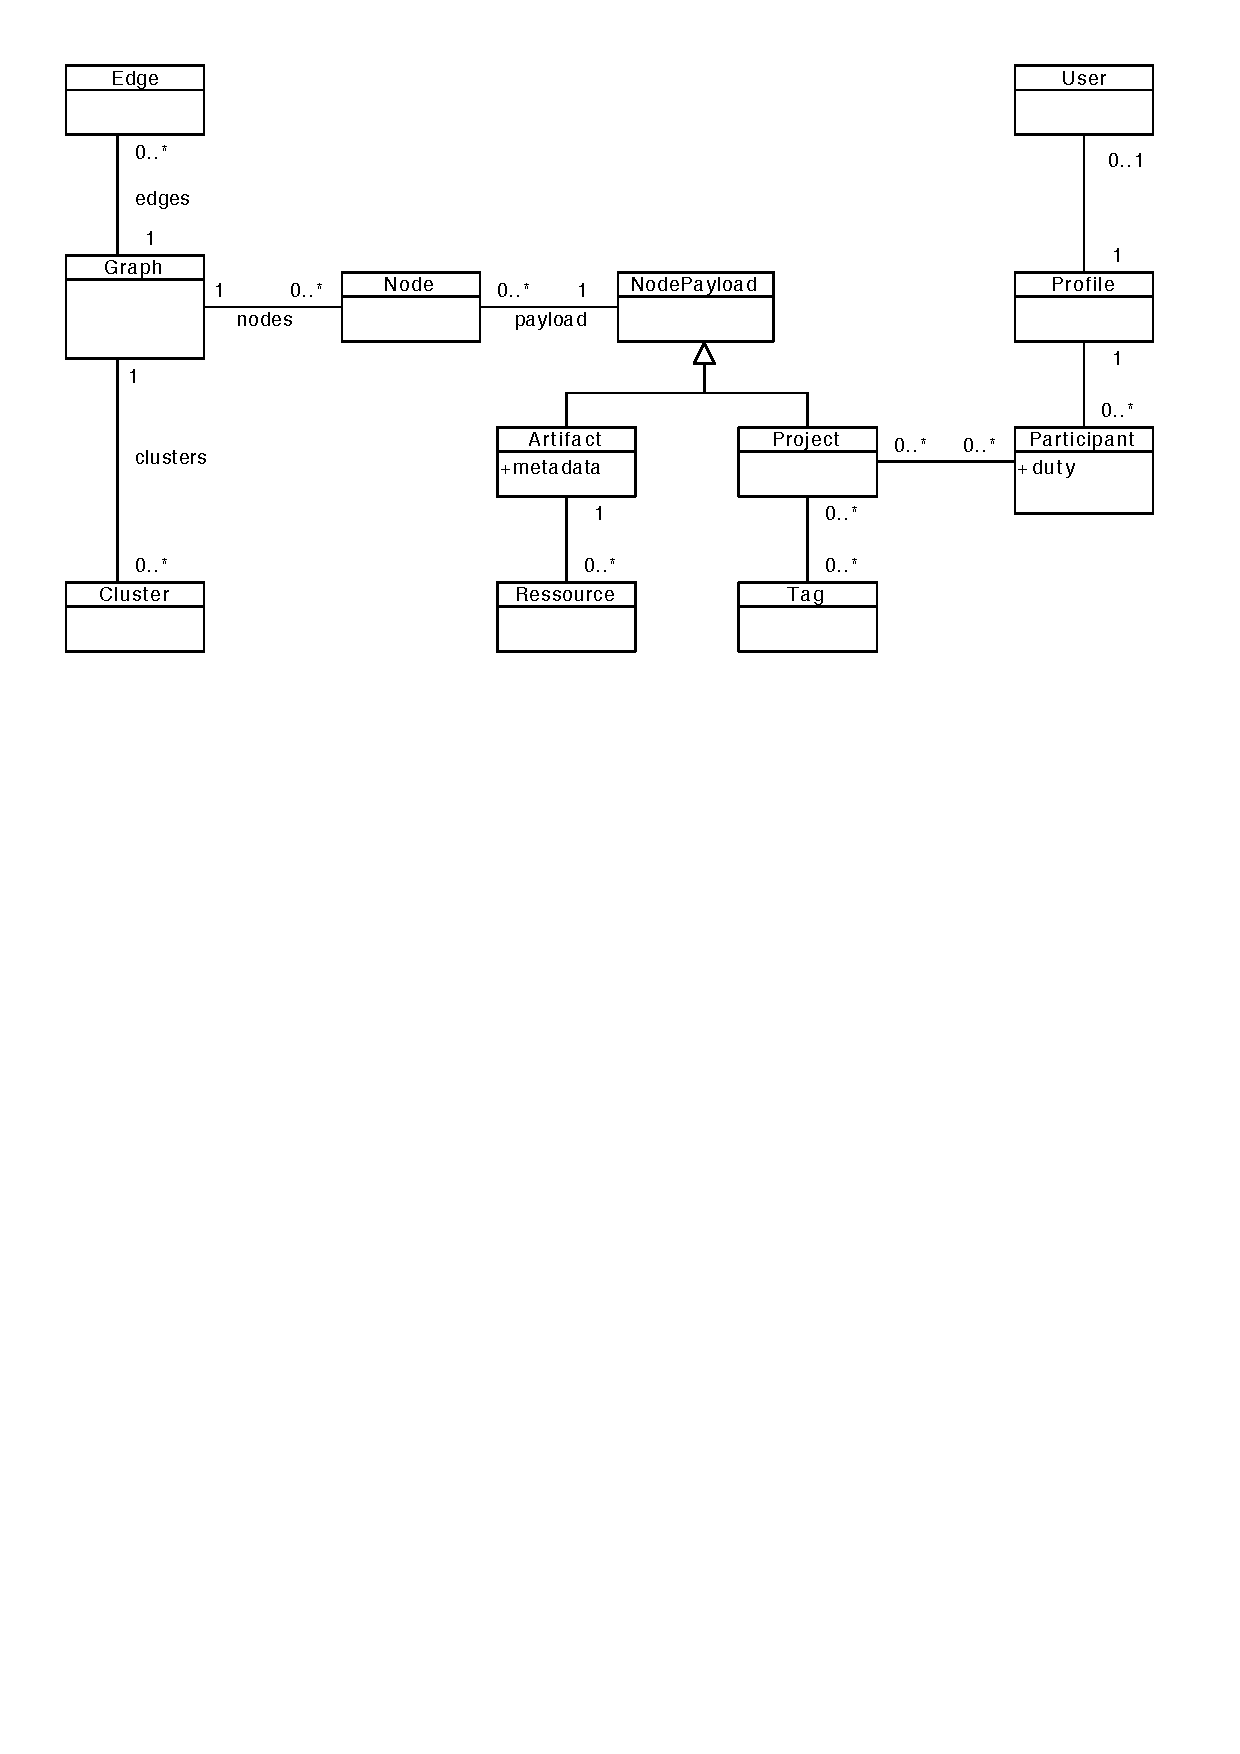
\includegraphics[width=1.0\textwidth]{img/models.pdf}  
   \caption{Ausgewählte Datenmodelle und ihre Assoziationen}
  \label{fig:models} 
\end{figure}

\subsection{Datenmodell für Graphen}
Ein Graph wurde als gerichteter Graph mit jeweils einer Liste für Knoten, Kanten und Cluster modelliert. Knoten und Kanten entsprechen denen aus der Graphentheorie bekannten Strukturen. Als konzeptionelle Referenz für den Aufbau eines Graphen dient \cite[p.~531]{corman}. Cluster wurden eingeführt, um Nutzern die Möglichkeit zu geben, Knoten zu gruppieren und \tete{Tags}\footnote{Als Tags bezeichnet man Schlagwörter, welche zu den Metadaten eines Objektes hinzugefügt werden.} hinzuzufügen. Ein Objektdiagramm eines Graphens wird in der Abbildung \ref{fig:graph-bsp} im Anhang gezeigt.

In der Datenbank sind für den \tete{Payload} eines Knotens nur Referenzen abgelegt. Der Payload beschreibt dabei den eigentlichen Inhalt eines Knotens, z.B. ein Projekt oder ein Artefakt. Wenn der Graph über die REST-Schnittstelle ausgeliefert wird, dann wird diese Referenz auf den \tete{NodePayload} mit dem eigentlichen Inhalt des Knotens ersetzt. Dies verringert den Speicherbedarf des Graphs in der Datenbank und verhindert das mehrfache Speichern des Payloads.

\subsubsection{Versionierung}

Um die Veränderungen an einem Graph nachverfolgen zu können, wurde eine Versionierung für Graphen eingeführt. Dadurch, dass nur Referenzen auf den Inhalt eines Knotens gespeichert werden, ist die Größe eines Graphens vergleichsweise gering. Aus diesem Grund ist es möglich, alle Versionen eines Graphens in der Datenbank abzulegen. Zur Identifizierung bekommt ein Graph eine Gruppe (\tete{group}) zugewiesen. In einer Gruppe liegen die verschiedenen Versionen eines Graphen. Zusammen mit der Versionsnummer \tete{version}, welche bei jedem Update inkrementiert wird, bildet die Gruppe einen Schlüssel.

\subsubsection{Updaten eines Graphen}

Um ein Graphen-Update ausführen zu können, wurde die Spezifikation von JSON-Patch\footnote{JavaScript Object Notation Patch, \url{http://tools.ietf.org/html/rfc6902} (Zugriff 15.06.13)} zur Veränderung von JSON-Objekten gewählt. Diese definiert eine JSON-Struktur, um ein gegebenes Objekt durch die Anwendung einer geordneten Folge von Änderungen in einen neuen Zustand zu überführen. Das Patch-Objekt ist ein JSON-Array, dessen Elemente als Operationen auf das zu verändernde JSON-Objekt angewendet werden sollen. Die definierten Operationen sind das Hinzufügen, Testen, Entfernen, Ersetzen, Verschieben und Kopieren von Attributen.

Alternativ bestünde die Möglichkeit, bei jeder Änderung den kompletten, geänderten Graphen zu senden. Da es sich hier um kleine Objekte handelt, wäre der Mehrbedarf an Bandbreite vertretbar. Für den Mehrnutzerbetrieb ist allerdings die Verwendung von JSON-Patch vorteilhaft, denn durch das explizite Senden der Änderungen ist ein Zusammenführen gleichzeitiger Änderungen von unterschiedlichen Quellen einfacher. Im Hinblick auf ebendiesen Vorteil wurde in Project-Zoom JSON-Patch verwendet. Die Implementierung im Frontend ist in \cite{bp-norman} näher beschrieben.

\subsection{Datenmodell für Artefakte}

\tete{Artefakte} werden durch externe Konnektoren gefunden und anschließend durch den Backend-Core in der Datenbank abgelegt, wo alle Informationen enthalten sind, die charakteristisch für das jeweilige Artefakt sind. Eine Besonderheit zeigt sich im Feld \tete{metadata}. Hier können alle Informationen eines Konnektors gespeichert werden, die keinem allgemeinen Feld zugeordnet werden können. Durch diese Speicherung von Informationen, die zwar im Moment für die Anwendung irrelevant sind und nicht von allen Konnektoren geliefert werden können, vermeidet man einen Informationsverlust. Bei der Weiterentwicklung der Anwendung können dann Informationen aus diesen Metadaten extrahiert und als eigenständige Felder verwendet werden. 

Zu einem Artefakt sind verschiedene \tete{Ressourcen} abgelegt. Eine Ressource bezieht sich hierbei auf die digitale Repräsentation eines Artefakts. Das heißt, dass es zu jedem Ressourcenobjekt in der Datenbank eine zugehörige Datei im Dateisystem gibt. Beispielsweise ist die originale Datei eine Ressource, generierte Thumbnails sind weitere. Das Feld \tete{typ} beschreibt die Art der Ressource und erlaubt einem Client die differenzierte Behandlung unterschiedlicher Typen.  

\subsection{Datenmodell für Nutzer}

Neben Artefakten können durch einen externen Konnektor auch Profile gesammelt werden. Diese Profile bestimmen die Zugriffsrechte eines Nutzers. Der mit einem Profil verknüpfte User enthält die Anmeldeinformationen, welche für die Authentifizierung benötigt werden. Ein User wird erst dann zu einem Profil assoziiert, wenn sich ein Nutzer mit der im Profil angegebenen E-Mail-Adresse für Project-Zoom registriert. Aus diesem Grund ist es auch nur Nutzern erlaubt sich zu registrieren, für die bereits ein Profil existiert.

Die Abspaltung des Users als Container für die Authentifizierungsinformationen vom Profil hat weiterhin den Vorteil, dass diese Informationen nicht über einen Konnektor geändert werden können. Wäre das der Fall, so könnte ein Angreifer die Log-In-Informationen für Project-Zoom durch das Verändern von Daten in einem Konnektor so anpassen, dass er Zugriff auf den Nutzer-Account bekommt.

%--------------------------------------------------------------------------------------------------------------------------------------------

\section{Data-centric Design}
\label{sec:dcd}
In diesem Kapitel wird die grundlegende Architektur der Anbindung eines persistenten Speichers im Core von Project-Zoom näher erläutert. Das gewählte Design hat vorrangig Auswirkungen auf die Art und Weise, wie der Code für Datenmodelle geschrieben wird, erstreckt sich aber als Betrachtungsweise über die gesamte Architektur. Zuerst wird das verwendete data-centric Design näher beschrieben und mit alternativen etablierten Formen der Datenbankanbindung verglichen. Im Kapitel \ref{sec:umsetzung_dcd} wird näher auf die Umsetzung des Designs in Project-Zoom eingegangen.

\subsection{Motivation}
\label{sec:dcdmotivation}
Das JSON Coast-To-Coast Design als Umsetzung des data-centric Designs wurde erstmals zusammenhängend und mit Beispielen unterlegt von Pascal Voitet in \cite{jctc} dargestellt. Voitet ist Mitwirkender am Open-Source-Projekt \tete{Play}\footnote{Play Framework, \url{http://playframework.com} (Zugriff 29.06.13)} und Autor von Scala-Bibliotheken (\tete{play-reactivemongo}\footnote{ReactiveMongo, \url{ https://github.com/zenexity/Play-ReactiveMongo} (Zugriff 15.06.13)}, \tete{play-autosource}\footnote{Play Autosource, \url{ https://github.com/mandubian/play-autosource} (Zugriff 15.06.13)}). 

Ein Backend für eine Webapplikation ist zunehmend eine Verbindung zwischen verschiedenen anderen Backends und Frontends. Diese Entwicklung geht auf die Bereitstellung von APIs für viele große und kleine im Web verfügbare Dienste zurück. Anwendungen, welche Daten vorrangig aus anderen Quellen aggregieren, sind zum großen Teil mit der Datenmanipulation beschäftigt. Hier bietet sich ein data-centric Design an. Grundlegend für das Design sind dabei folgende Entwicklungen: Zum einen das Aufstreben von NoSQL-Datenbanken und zum anderen asynchrone Datenbanktreiber mit einfachen Methoden zur JSON-Manipulation.

\subsubsection{NoSQL}
Die Entwicklung der Datenbankmanagementsysteme beschränkte sich viele Jahre auf die Optimierung und Verbesserung bestehender relationaler Datenbankmodelle. Im Jahr 1998 kam der Term \tete{Not-only SQL} (NoSQL) auf (vgl. \cite{storage-solutions}). Heute gibt es verschiedene etablierte Datenbanken, die keine reinen SQL-Datenbanken mehr sind, wie beispielsweise MongoDB\footnote{MongoDB, \url{http://mongodb.org} (Zugriff 17.06.13)}, Apache CouchDB\footnote{Apache CouchDB, \url{http://couchdb.apache.org} (Zugriff 17.06.13)} und Apache Cassandra\footnote{Apache Cassandra, \url{http://cassandra.apache.org} (Zugriff 17.06.13)}.

NoSQL-Datenbanken sind vorteilhaft für ein data-centric Design, da zur Umsetzung eines Datenflusses (vgl. Abbildung \ref{fig:dataflow}) eine Ähnlichkeit des Datenbank- und Clientformats vorliegen muss. Diese Ähnlichkeit liegt zum Beispiel bei BSON und JSON vor und verhindert somit die Notwendigkeit einer Konvertierung.

\subsubsection{Datenbanktreiber}
\label{sec:reactive}
Für die Anbindung von relationalen Datenbanken gibt es in Java die Java Database Connectivity (JDBC). Diese Schnittstelle abstrahiert über Datenbanken und deren Treiber, indem eine einheitliche API angeboten wird. Ausgerichtet ist JDBC auf relationale Datenbanken (vgl. \cite{reese2000database}).

Um NoSQL-Datenbanken anzubinden, benötigt man, wie bei JDBC, einen eigenen Treiber. Der Unterschied ist, dass es hier keine Abstraktionsebene über verschiedene NoSQL-Datenbanken gibt. Dies liegt vorrangig an der sich stark unterscheidenden Struktur der einzelnen Speichersysteme\footnote{Die gängigsten Formate sind dokumentenbasierte Speicher oder einfache Schlüssel-Wert-Speicher (vgl. \cite{nosql-databases}), es gibt jedoch noch eine Reihe weiterer Speichersysteme.}. Die unterschiedlichen NoSQL-Datenbanken sind jeweils speziell auf eine bestimmte Aufgabe ausgerichtet, wie z.B. auf Durchsatz, verteilte Umgebungen oder flexible Datenschemas. 

\tete{ReactiveMongo} ist ein Beispiel für einen asynchronen Datenbanktreiber für MongoDB. Die Vorteile eines asynchronen Treibers liegen auf der Hand: Für jede synchrone Datenbankabfrage wird normalerweise ein Thread verwendet, der bis zur Antwort blockiert ist. Bei mehreren Datenbankabfragen pro Request werden bei Last viele Threads benötigt, um Datenbankabfragen auszuführen. Asynchrone Treiber umgehen dieses Problem, indem sie Threads, welche Datenbankabfragen ausführen, nicht blockieren. Für dieses Konzept ist es notwendig, Platzhalter einzuführen. Diese ersetzen das Ergebnis, solange es noch nicht vorhanden ist.

\begin{lstlisting}[label=lst:asyncaccess, caption=Funktionssignatur für asynchronen Datenbankzugriff]
def findById(bid: BSONObjectID): Future[Graph] = {
  collection.find("_id" -> bid)
}
\end{lstlisting}
 
Im Quelltext \ref{lst:asyncaccess} zeigt die Funktionssignatur den Rückgabetyp \tete{Future[Graph]}. \tete{Future} ist hierbei ebendieser Platzhalter für ein Ergebnis, welches noch nicht existiert. Futures basieren dabei auf einem Konzept, welches in \cite{future-concept} beschrieben ist. Um auf das Ergebnis eines Futures zu reagieren, können verschiedene \tete{Callbacks} festgelegt werden.

Die Verwendung eines asynchronen Treibers ist vor allem im Hinblick auf das zu implementierende, asynchrone Eventsystem sinnvoll und von Vorteil. 

\subsubsection{Manipulation von JSON}
Das data-centric Design basiert auf der Idee der direkten Manipulation von Daten. Für eine Umsetzung des data-centric Designs mit Hilfe von JSON benötigt man somit eine Bibliothek, welche die Möglichkeit bietet, JSON zu transformieren und zu validieren.
 
Eine solche Bibliothek, welche das Validieren, Transformieren und Serialisieren erlaubt, ist Play-JSON. Ein Beispiel, wie solch eine Transformation und Validierung aussieht, ist im Anhang im Quelltextauszug \ref{app:jsonbsp} zu sehen. Dort wird ein JSON-Objekt erzeugt, welches anschließend zuerst transformiert wird, indem das Attribut \tete{role} angehangen wird, und danach validiert wird. Bei der Validierung wird überprüft, ob der Nutzer über 18 Jahre alt ist.

\subsection{Idee hinter data-centric Design}
Das Ziel im data-centric Design ist die direkte Manipulation von Daten. Der Fokus des Designs liegt dabei sowohl auf der Datenmanipulation als auch auf dem Datenfluss. Wie bereits im Abschnitt \ref{sec:dcdmotivation} beschrieben, sind Webapplikation-Backends immer häufiger Knotenpunkte in einem mehrere Server durchlaufenden Datenfluss. Ein Teil dieses Datenflusses, die Kommunikation des Backends mit der Datenbank und dem Client, ist in Abbildung \ref{fig:dataflow} dargestellt. 

\begin{figure}[h]   
  \centering     
  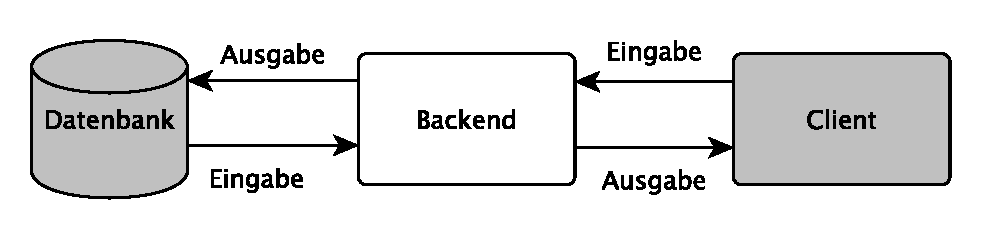
\includegraphics[width=0.8\textwidth]{img/dataflow_dcd.pdf}  
   \caption{Datenfluss zwischen Datenbank, Backend und Client}   
  \label{fig:dataflow} 
\end{figure}

In diesem Datenfluss soll es keine implizite Umwandlung der Daten in Objekte der Programmiersprache\footnote{Es ist bekannt, dass die Repräsentation der Daten des Datenflusses ebenfalls in Objekten der Programmiersprache erfolgt (beispielsweise JSON-Objekte). Mit dem Ausdruck ist die Überführung der Daten aus einem allgemeinen Modell (z.B. JSON) in eine spezifische Objektdarstellung (z.B. ein Objekt einer User-Klasse) gemeint.} geben. Für ein einfaches Durchleiten der Daten aus der Datenbank zum Client oder von einer anderen Webressource zum Client ist eine Umwandlung nicht notwendig oder sinnvoll. 

Im Gegensatz zu anderen Modellen ist die Abstraktion von der Datenquelle kein Ziel des data-centric Designs. Das Festlegen auf eine Datenquelle bei der Entwicklung eines Systems erlaubt die Verwendung aller Funktionen, die diese Datenquelle zur Verfügung stellt. Beispielsweise erlaubt MongoDB die Verwendung sogenannter \tete{Capped Collections}\footnote{Weitere Informationen zu Capped Collections z.B. auf \url{http://docs.mongodb.org/manual/core/capped-collections/} (Zugriff 20.06.13)}, welche auf hohen Durchsatz optimiert sind. Diese verhalten sich wie eine zirkuläre Queue mit begrenzter Größe. Viele Datenbanken besitzen spezielle, stark angepasste Funktionen, auf die jedoch bei der Verwendung von allgemeinen Datenbank-APIs (z.B. JDBC) meist nicht zugegriffen werden kann. Ein Nachteil dieser engen Kopplung ist, dass der Austausch der Datenquelle dadurch schwieriger ist. 

Eine Deserialisierung der Daten in Objekte ist für komplexe Business-Logik von Vorteil. Statische Datenmodelle sollten immer dann verwendet werden, wenn die Manipulation der Daten kompliziert wird. Hier kommt der Nachteil von dynamischen Speicherstrukturen zum Vorschein, denn sobald es nicht mehr darum geht ein JSON-Objekt zu Transformieren oder zu Validieren, sondern auf einzelne Attribute zuzugreifen, muss dieses Attribut immer einzeln deserialisiert werden. Das schließt die Berücksichtigung der Fehlerfälle, wie dem Fehlen des Attributes oder dem Vorhandensein des falschen Typs, mit ein. Aus diesem Grund ist an dieser Stelle eine Umwandlung in ein Objekt der Programmiersprache vor der Verwendung sinnvoll. Ebenfalls notwendig ist diese Konvertierung bei der Verwendung der meisten externen Bibliotheken.

Nach Voitet sollten statische Datenmodelle also nicht vergessen, sondern nur dann genutzt werden, wenn sie notwendig sind. Einfache und dynamische Strukturen sollten so oft es geht erhalten bleiben (vgl. \cite{jctc}).

\subsection{Abgrenzung zur objektrelationalen Abbildung}
Das \tete{Object-relational Mapping} (ORM) wird auch als \tete{All-Model-Approach} bezeichnet. Hierbei erfolgt die Kommunikation mit der Datenbankschnittstelle über Objekte der Programmiersprache. Abfragen an die Datenbank resultieren in Objekten der Programmiersprache. Der Fokus der objektrelationalen Abbildung liegt in der Überführung von Objekten der objektorientierten Programmierung in ein relationales, tabellenorientiertes Schema (vgl. \cite{wambler}). 

\begin{figure}[h]   
  \centering     
  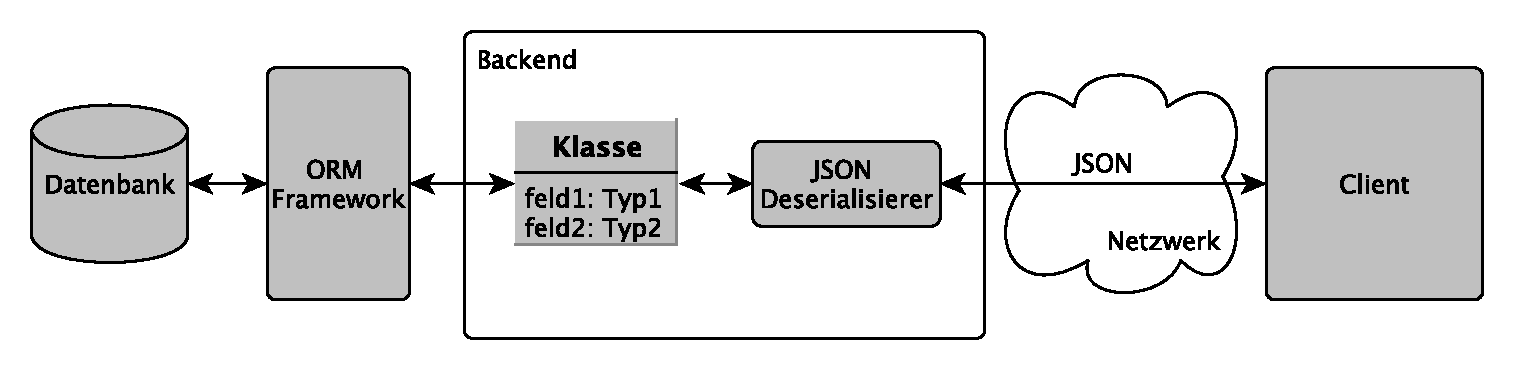
\includegraphics[width=1.0\textwidth]{img/dataflow_orm.pdf}  
   \caption{Datenfluss einer Applikation bei Verwendung eines ORM-Frameworks}   
  \label{fig:orm} 
\end{figure}

Der wichtigste Vorteil eines Frameworks für die objektrelationale Abbildung liegt in der Abstrahierung von der Datenbank. Für die Business-Logik gibt es keinen Unterschied zwischen Objekten aus der Datenbank und Objekten der Programmiersprache. Die Datenbank kann meist ohne Änderungen an der Applikation ausgetauscht werden.

\FloatBarrier
\subsubsection{Objektrelationale Unverträglichkeit}
\label{sec:unvertraeglich}
Ein ORM bringt konzeptionelle Probleme mit sich. Diese werden in der Literatur (vgl. \cite{ireland2009classification}) in der Regel als \tete{Object-relational Impedance Mismatch} (ORIM) bezeichnet. Die objektrelationale Unverträglichkeit resultiert aus den Unterschieden im zugrundeliegenden Konzept, sowie aus Differenzen in der Darstellung und den Erwartungen des Entwicklers (vgl. \cite{bowers}).

Folgende Herausforderungen ergeben sich für die praktische Arbeit mit einem ORM:

\begin{itemize}
  \item Die Abbildung der Assoziationen zwischen den Objekten ist komplex. Es müssen One-to-One, One-to-Many und Many-to-Many Abhängikeiten ins relationale Schema übertragen werden.
\item Ein weiterer zentraler Punkt ist die Abbildung von Hierarchien und Vererbungen aus der objektorientierten Programmierung in das relationale Datenmodell. 
\item Innerhalb des ORM muss es ein Objekt-Caching geben. Dieses ist notwendig um die Illusion zu erzeugen, dass es sich um ein Objekt der Programmiersprache handelt. Denn wird ein Objekt mehrmals aus der Datenbank abgefragt, so muss ein referenzgleiches Objekt zurückgegeben werden (vgl. \cite{inappropriate-abstractions}).
\item Der Entwickler muss die ORM-Limitierungen, die sich aus dem ORIM ergeben, akzeptieren. Die Probleme müssen somit bekannt sein, um sie bereits bei der Datenmodellierung zu umgehen (vgl. \cite{vietnam}). 
\end{itemize}

Ted Neward, Autor von „The Busy Java Developers Guide to Scala“ \cite{busy-to-scala}, macht den frühen Erfolg von objektrelationalen Abbildungen und die Erleichterungen, welche die ersten ORMs mit sich brachten, dafür verantwortlich, dass zum Teil ORMs verwendet werden, ohne deren Limitierungen zu beachten. Das wiederum führt zu einem erheblichen Mehraufwand an Zeit und Energie für die Erhaltung und Anpassung an alle Nutzungsfälle (vgl. \cite{vietnam}).

\subsubsection{Unterschiede zum data-centric Design}
Das data-centric Design ist viel stärker an die Datenbank gebunden und deren Austausch ist deutlich schwieriger. Dies sorgt dafür, dass keine Illusion einer abstrahierten Datenbank entsteht. Da das data-centric Design ein Ansatz mit funktionalem Hintergrund ist, sind die Datenstrukturen zur Laufzeit in der Regel unveränderbar\footnote{Die hier beschriebene Unveränderbarkeit bezieht sich auf die in der funktionalen Programmierung übliche Bedeutung. Die Struktur eines Objektes ist zur Entwurfszeit beliebig veränderbar. Zur Laufzeit können den Attributen eines Objektes nach Erstellung dessen keine neuen Werte mehr zugewiesen werden. Der Zustand des Objektes ist somit unveränderbar (vgl. \cite[p.~181]{programmieren-in-scala}).}. Ein Caching zur Sicherung der Objektidendität ist daher nicht notwendig. Die Objektgleichheit ist in diesem Fall über Wertgleichheit definiert (vgl. Scala Case-Klassen in \cite{scala-case-class}). Im Gegensatz zum ORM muss sich der Entwickler beim data-centric Design selbst mit der Darstellung und Umwandlung seiner Daten in das Datenbankformat beschäftigen. Durch die Verwendung einer objekt- oder dokumentenbasierten Datenbank ist diese Umwandlung einfacher und mit weniger Problemen behaftet, als eine Konvertierung in ein relationales Schema.

\subsection{Abgrenzung zu Datenzugriffsobjekten}
Implementierungen von Datenzugriffsobjekten, in der englischsprachigen Literatur \tete{Data Access Object} (DAO) oder \tete{Data Access Procedure}, basieren auf dem \tete{Data Access Object}-Pattern (vgl. \cite{j2ee-pattern}).  Das Pattern hat das Ziel, den Datenzugriff und die Datenmanipulation in einen separaten Layer auszulagern. Daraus ergibt sich eine Kapselung der Datenbankzugriffe an einem Ort der Applikation. Bei der Umsetzung gibt es die Möglichkeit, ein DAO zur Abstraktion der Datenbank als Ganzes zu verwenden oder für jede einzelne Datenbankstruktur ein DAO anzulegen.

Der Hauptfokus liegt in der Abstrahierung der Datenbank. Bei Änderungen an der Datenquelle müssen in der Regel nur die Datenzugriffsobjekte angepasst werden, denn der Anwendungscode bleibt im Allgemeinen unberührt. Die Serialisierung der Daten von den Strukturen der Anwendung in Strukturen der Datenbank ist nicht Aufgabe des DAO, sondern des \tete{Data Transfer Object} (DTO)\footnote{vgl. J2EE Patterns – Data Transfer Object \url{http://www.oracle.com/technetwork/java/transferobject-139757.html} (Zugriff 20.06.13)}.

Im DAO findet über einen Datenbanktreiber direkter Zugriff auf die Datenbank statt. Man kann das Datenzugriffsobjekt somit als Bindeglied zwischen Datenbank und Applikation sehen. Durch die direkte Kommunikation mit der Datenquelle können alle unterstützten Funktionen ausgenutzt werden. 

Sowohl DAO als auch ORM haben die Abstrahierung der Datenbank als Ziel. Im Gegensatz zum DAO geht das ORM jedoch noch einen Schritt weiter und abstrahiert nicht nur über die Funktionen, welche durch die Datenbank zur Verfügung gestellt werden, sondern auch über die innere Struktur der Datenquelle. In der Regel bauen ORM-Implementierungen auf dem Data Access Object-Pattern und dem Data Transfer Object-Pattern auf.

\subsubsection{Unterschiede zum data-centric Design}
Das DAO-Pattern enthält, ähnlich dem data-centric Design, keine Serialisierung oder Deserialisierung von Objekten. Beide Designs können sehr gut zusammen verwendet werden. Der Datenfluss kann somit durch ein DAO realisiert werden, wodurch die Vorteile des Datenzugriffsobjektes, wie zum Beispiel eine stärkere Kapselung, genutzt werden. Voitet benutzt in seinen Beispielen kein DAO, sodass sich die Datenbankabfragen über den kompletten Quellcode verteilen. Während das bei Beispielapplikationen oder kleineren Anwendungen kein Problem darstellt, geht bei größeren Anwendungen mit vielen verschiedenen Datenmodellen schnell die Übersichtlichkeit verloren. Die Verwendung eines Datenzugriffsobjektes führt zu einem \tete{Single Point of Responsibility}\footnote{ Single Responsibility Principle (SRP), vgl. \cite[p.~339]{design-patterns}}
 und stärkt somit die Struktur des gesamten Projektes. 

\subsection{Grenzen des data-centric Designs}
Das data-centric Design eignet sich sehr gut für \tete{Create-Read-Update-Delete} (CRUD)-Anwendungen. Dort liegt der Fokus auf der Datenmanipulation, was zum Grundsatz des Designs von Project-Zoom passt.

Es erfolgt eine explizite Bindung an das Datenmodell. Durch die Nähe zur Datenquelle können spezifische Fähigkeiten einer Datenquelle genutzt und Anfragen effektiver gestaltet werden. Die dynamischen Strukturen des Datenmodells ermöglichen eine leichte Veränderbarkeit des Modells sowie einfache Verknüpfungen zwischen Daten.

Grenzen sind dem data-centric Design vor allem durch die Business-Logik gesetzt. Durch die dynamischen Strukturen im Design ist der Code meist komplizierter und länger.

Ohne die Verwendung eines DAO gibt es in diesem Design keinen Single point of responsibility für Datenbankzugriffe. Das erschwert wiederum Änderungen am Schema, da diese zu unvorhergesehenen Problemen an anderen Stellen im Anwendungsquelltext führen können. Aus diesem Grund sollten bei diesem Design ein oder mehrere Datenzugriffsobjekte verwendet werden. Ein weiterer Vorteil bei der Verwendung eines DAO ist, dass die Datenquelle durch die Zentralisierung der Datenbankanfragen im Datenzugriffsobjekt deutlich leichter ausgetauscht werden kann.

%--------------------------------------------------------------------------------------------------------------------------------------------

\section{Eventsystem}
In der Anforderung \ref{itm:f2} wurde festgelegt, dass die von den Teams erstellten Dokumente aus der jeweiligen \gls{Box} für die Studierenden in Project-Zoom zur Verfügung stehen sollen. Diese Verfügbarkeit soll schnellstmöglich nach Hinzufügen einer neuen Datei zur \gls{Box} gegeben sein (siehe Anforderung \ref{itm:nf2}). Hierfür ist es sinnvoll ein asynchrones System zu bauen.  Neben der Anbindung von \gls{Box} ist für die Zukunft auch der Zugriff auf Facebook, Dropbox und Netzwerkdateisysteme vorgesehen. Es zeigt sich, dass ein paralleles, unabhängiges Abfragen der einzelnen Dienste notwendig ist.

Ein Eventsystem basiert auf dem Prinzip des Abonnierens und Veröffentlichens von Nachrichten und modelliert eine Eine-zu-Viele-Relation. Ein sogenannter \tete{Publisher} sendet seine Events, welche anschließend vom \tete{Dispatcher} an die \tete{Subscriber} verteilt werden. Die Subscriber können dieses Event schließlich abarbeiten (vgl. \cite[p.~327]{gang-of-four}). Das Publisher-Subscriber Modell kann sowohl synchron als auch asynchron implementiert werden. Bei einer asynchronen Umsetzung wird ausgenutzt, dass der Sender beim Emittieren einer Nachricht sofort sequentiell weiterarbeiten kann und die Bearbeitung des Events nicht abwarten muss.

\begin{figure}[h]  
  \centering     
  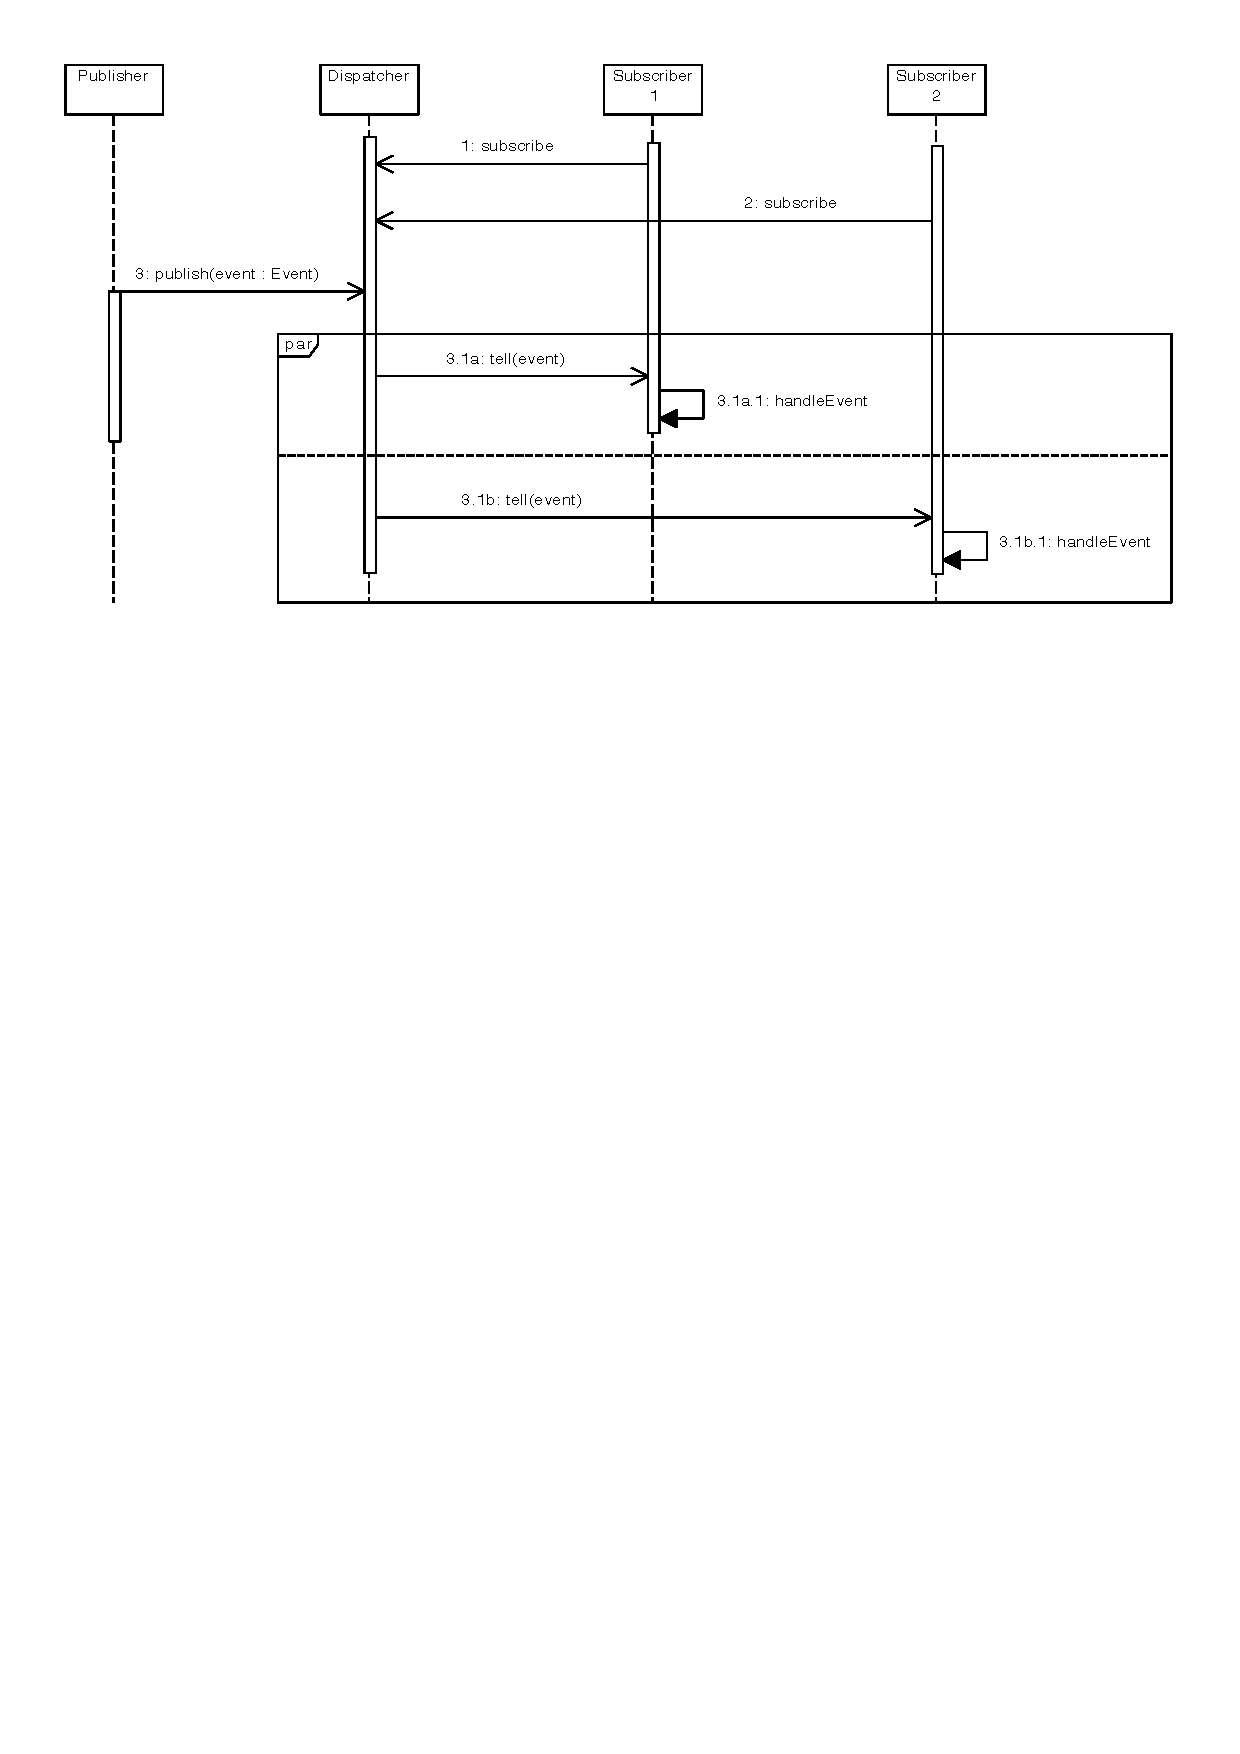
\includegraphics[width=1.0\textwidth]{img/eventsystem.pdf}  
   \caption{Funktionsweise des Eventsystems an einem Beispiel}   
  \label{fig:event-system} 
\end{figure}

Die parallele Abarbeitung von verschiedenen Aufgaben ist ein wichtiger Bestandteil von Project-Zoom. Ein Beispiel hierfür ist das Erzeugen von Thumbnails, was bei größeren Dateien eine gewisse Zeit in Anspruch nehmen kann. Diese Thumbnails werden für jedes durch einen Konnektor gefundene Artefakt erzeugt. Während der Thumbnailerzeugung muss die Webapplikation weiterhin Client-Anfragen beantworten können, weswegen die Thumbnailgenerierung ausgelagert wurde.

Ebenfalls von Bedeutung ist die Ausfallsicherheit. Der Ausfall einer einzelnen Komponente darf die Stabilität des Gesamtsystems nicht beeinträchtigen. Eine falsch konfigurierte OpenOffice-Anbindung, welche der Thumbnailgenerator benötigt (vgl. \cite{bp-dome}), darf, selbst wenn der Thumnailerzeuger nicht mehr in der Lage ist zu arbeiten, das System nicht zum Stillstand bringen.

Ein weiterer Vorteil ist die Flexibilität, die durch ein Publisher-Subscriber-Modell erreicht wird. Wenn eine neue Komponente eingebunden werden soll, so kann sich diese auf bereits emittierte Nachrichten abonnieren und somit auf Ereignisse im Gesamtsystem reagieren.

In Abbildung \ref{fig:event-system} ist der Aufbau eines Eventsystems zu sehen. Der Dispatcher ist die zentrale Komponente im Eventsystem, denn er verwaltet die Abonnements und verteilt die Events an die Subscriber. Diese Verantwortung stellt eine Schwachstelle im Eventsystem dar, es existiert ein \tete{Single Point of Failure}. Ein Ausfall kann durch die Vervielfältigung des Dispatchers vermieden werden, wobei eine gemeinsame Datenbasis für alle Dispatcher notwendig ist. 
